\section{Przegląd istniejących rozwiązań}

%------------------------------------------------

\begin{frame}
\frametitle{Robot Velma}
\begin{figure}
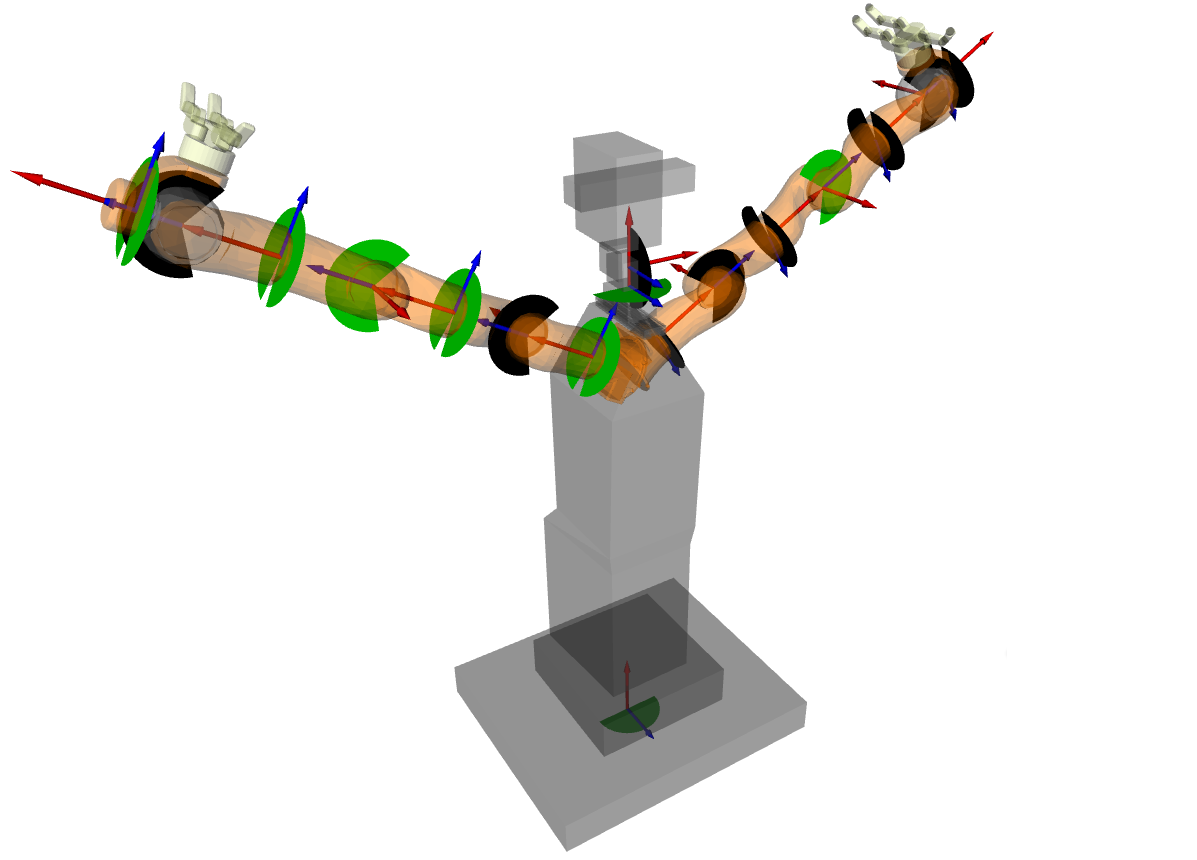
\includegraphics[scale=0.22]{./images/velma_joints.png}
\caption{Wizualizacja robota Velma z zaznaczonymi stopniami swobody \cite{docsVelma}}
\end{figure}
\end{frame}

%------------------------------------------------

\begin{frame}
\frametitle{Robot Velma}
Robot Velma składa się z \cite{docsVelma}:  
\begin{itemize}
	\item obrotowego korpusu
	\item dwóch manipulatorów KUKA LWR
	\item dwóch chwytaków BarrettHand
	\item szyi o dwóch stopniach swobody
\end{itemize}
\end{frame}

%------------------------------------------------

\begin{frame}
\frametitle{Struktura symulatora}

\end{frame}

%------------------------------------------------

\begin{frame}
\frametitle{Robot Velmobil}
\begin{figure}
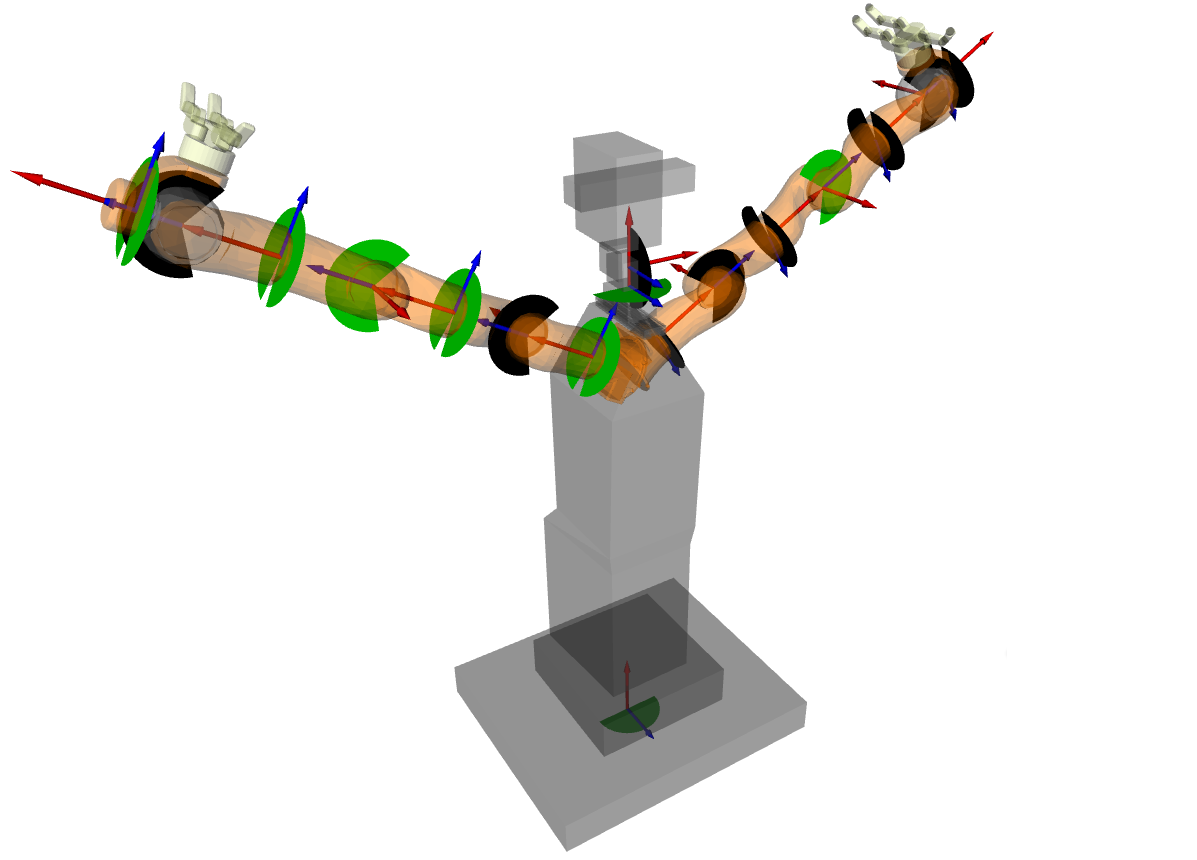
\includegraphics[scale=0.22]{./images/velma_joints.png}
\caption{Wizualizacja robota Velma z zaznaczonymi stopniami swobody \cite{docsVelma}}
\end{figure}
\end{frame}

%------------------------------------------------

\begin{frame}
\frametitle{Robot Velmobil}
Robot Velma składa się z \cite{docsVelma}:  
\begin{itemize}
	\item 4 koła szwedzkie
\end{itemize}
\end{frame}

%------------------------------------------------

\begin{frame}
\frametitle{Struktura symulatora}

\end{frame}